\begin{center}
\begin{picture}(\spaltenbreite,20)
\put(-4,10){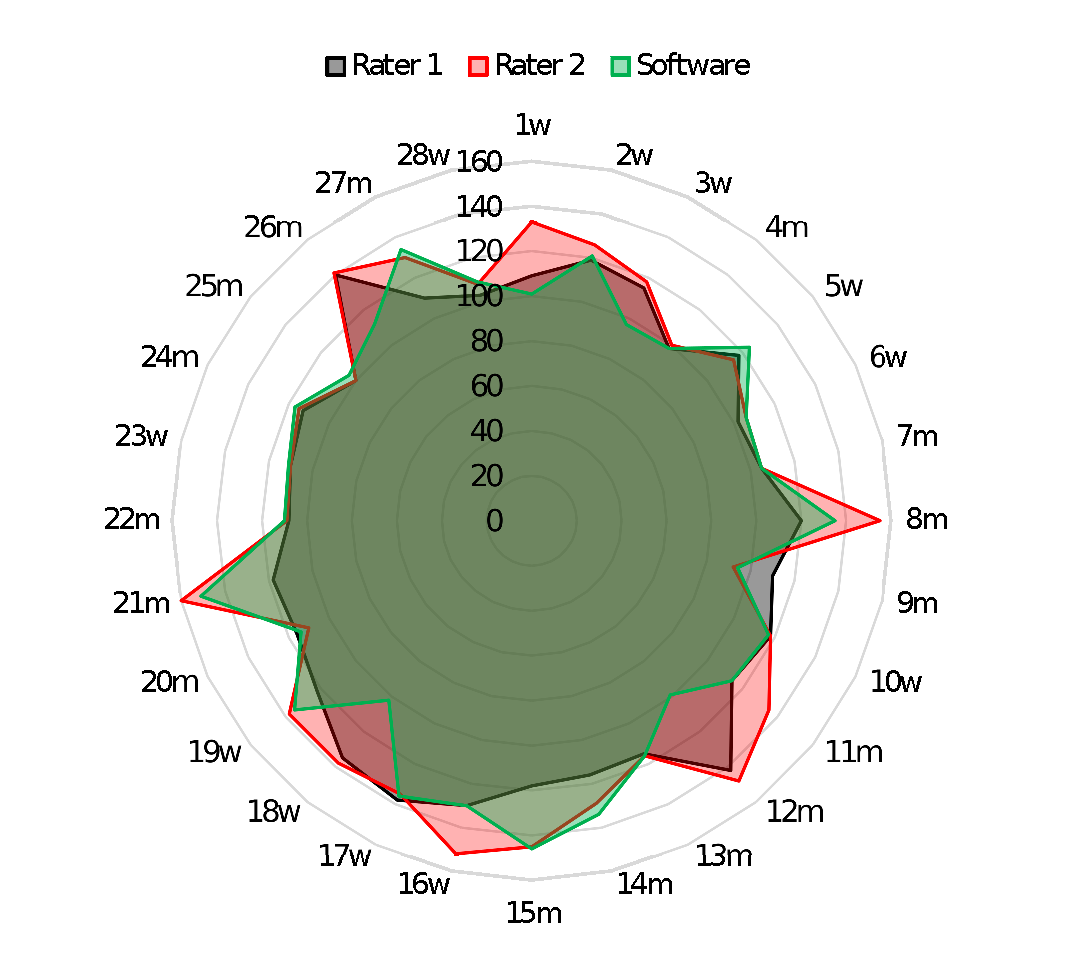
\includegraphics[width=110mm]{Bilder/v-slope_net.eps}}
\put(-0.8,9){\parbox{720pt}{{\bf \small a)} \small für V-Slope}}
\put(8,10){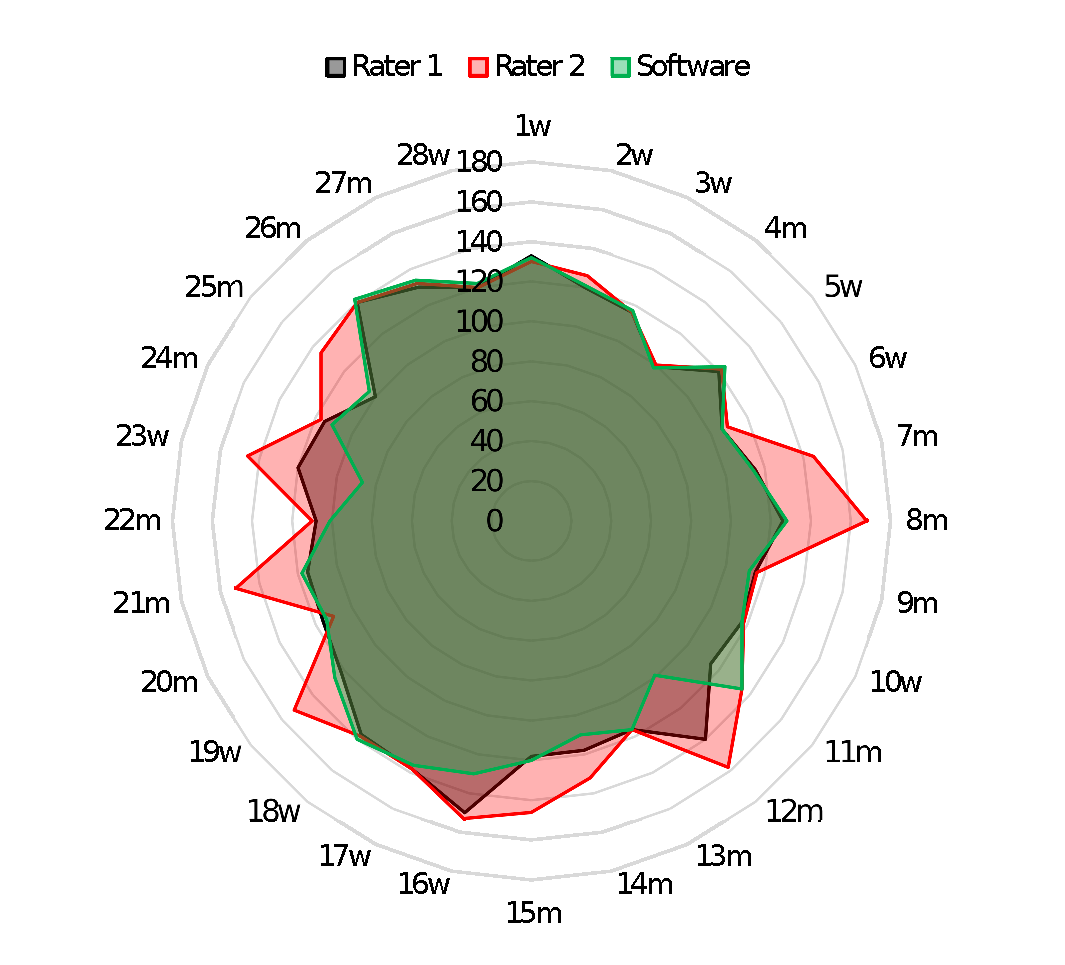
\includegraphics[width=110mm]{Bilder/eqo2_net.eps}}
\put(11.3,9){\parbox{720pt}{{\bf \small b)} \small für EQO\textsubscript{2}}}
\put(-4,-2){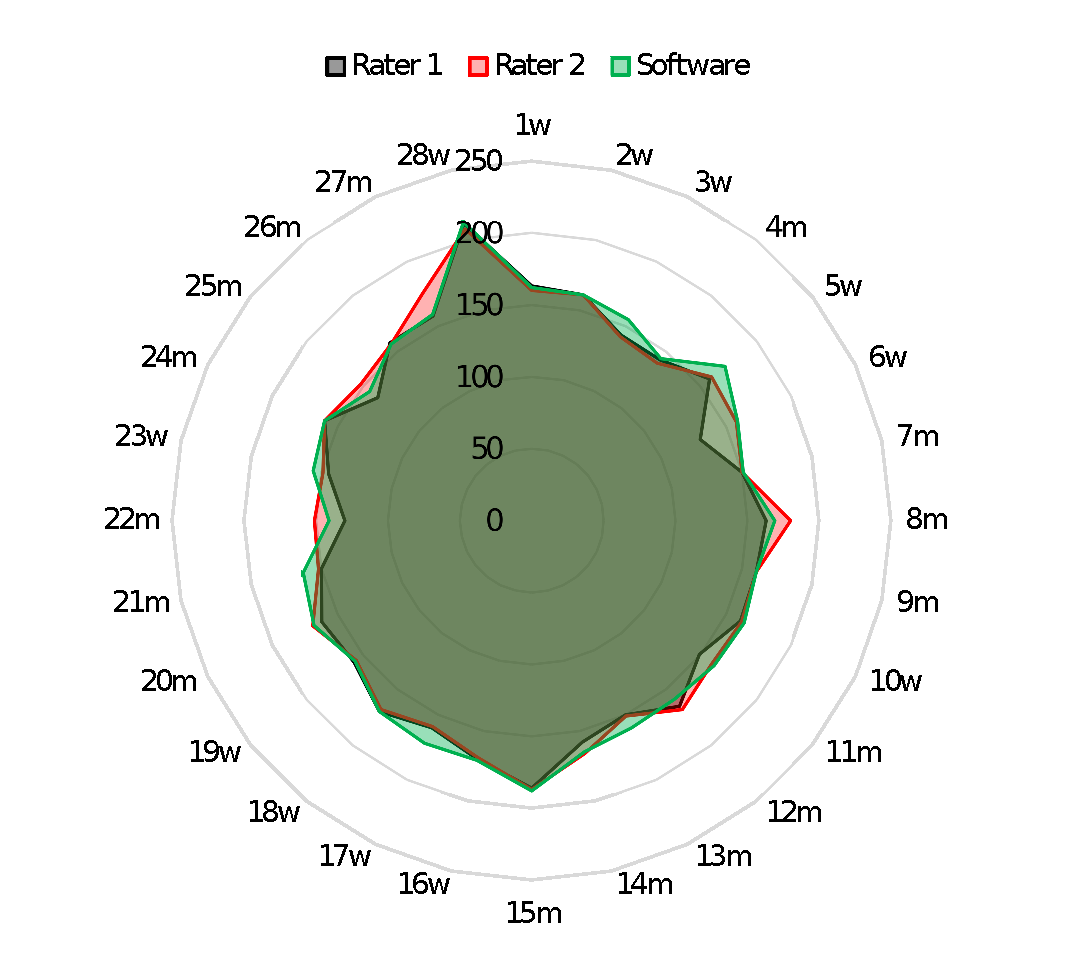
\includegraphics[width=110mm]{Bilder/eqco2_net.eps}}
\put(-0.7,-3){\parbox{720pt}{{\bf \small c)} \small für EQCO\textsubscript{2}}}
\put(8,-2){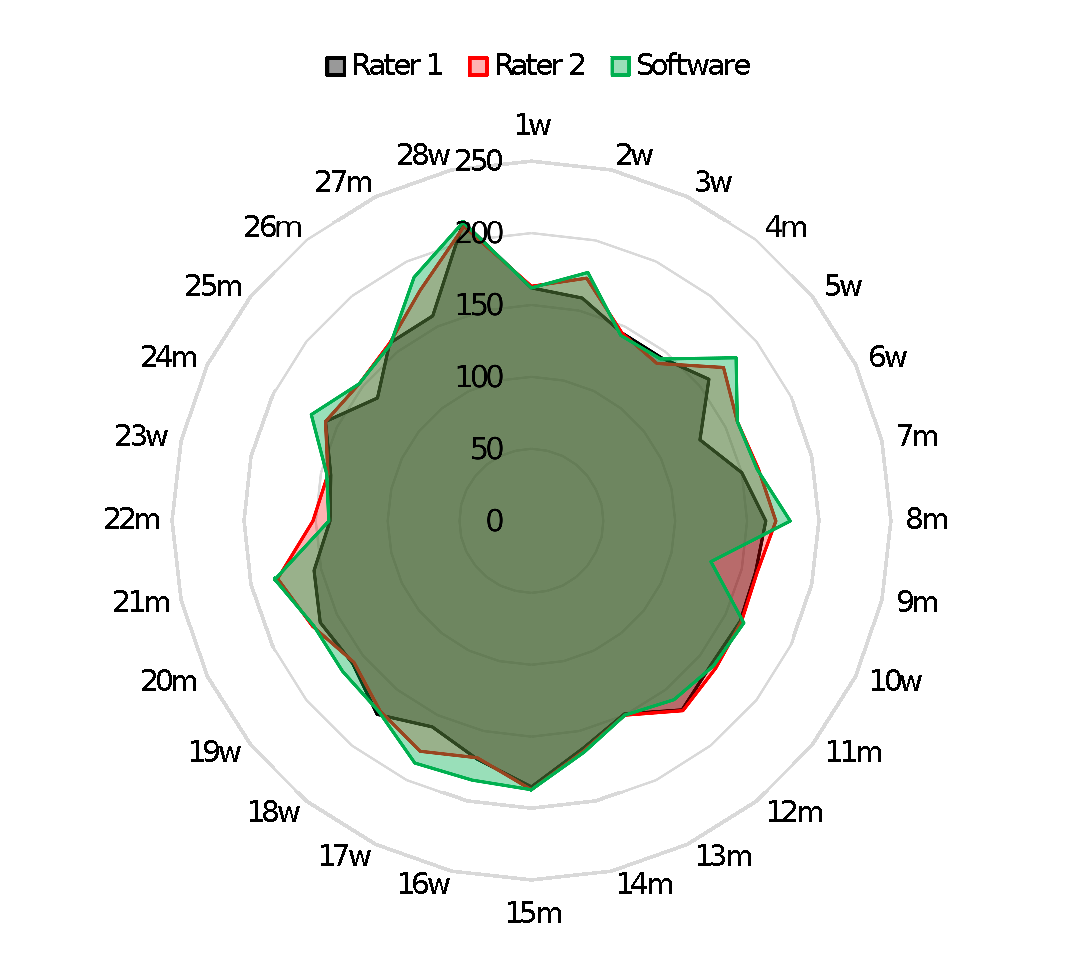
\includegraphics[width=110mm]{Bilder/vevco2_net.eps}}
\put(10.8,-3){\parbox{720pt}{{\bf \small d)} \small für \.{V}E/\.{V}CO\textsubscript{2}}}
\put(-0.85,-5){\parbox{720pt}{{\bf \small Abb. 3:} \small Verteilung der Ergebnisse für die Schwellen}}
\end{picture}
\end{center}
\vspace*{6.3cm}
Abb. 3 zeigt die unterschiedlichen Ergebnisse der Schwellenbestimmung der Rater und Software für die Probanden anhand der vier Methoden in Form von Netzdiagrammen.